\chapter{Conception du projet}
\minitoc
\clearpage
\section*{Intoduction}
Afin de créer une application respectant les besoins définis dans le cahier de charges, il faut d'abord passer par l'étape de conception. Cette étape permettra de décortiquer le cahier de charges et définir les acteurs, les cas d'utilisation, et finalement les différentes classes qui définiront les différents attributs de chaque entité qui interagit avec l'application.
\section{Spécification des besoins}
La première étape de la conception est de dégager les différents besoins de l'utilisateur. Ces besoins sont divisés en deux catégories: fonctionnels et non fonctionnels.
\subsection{Besoins fonctionnels}
\subsubsection{L'authentification}
Le client doit s'authentifier pour utiliser les différents services de l'application.
\subsubsection{Consulter les voitures disponibles}
Le client peux consulter les voitures disponibles selon sa position actuelle.
\subsubsection{Créer une réservation}
Le client peut créer un réservation en choisissant une voiture.
\subsubsection{Paiement en ligne}
Le client peut payer pour sa réservation à l'aide des méthodes de paiement en ligne.
\subsubsection{Signature numérique de contrat de location}
Le client peut signer son contrat de location en ligne en toute sécurité.
\subsubsection{Suivre la position de la voiture}
Le client peut suivre la position de la voiture louée en temps réel.
\subsubsection{Contacter le chauffeur}
Le client peut contacter le chauffeur de sa voiture louée par appel téléphonique ou messagerie instantannée.
\subsection{Besoins non fonctionnels}
\subsubsection{Interfaces graphiques}
L'utilisateur peut rapidement commencer à utiliser l'application sans difficulté à l'aide des interfaces graphiques claires et simples.
\subsubsection{Performances de l'application}
L'application ne doit pas présenter des imperfections en terme de rapidité et de fluidité en cours de son exécution.
\subsubsection{Maintenabilité et scalabilité}
L'application doit être simple à maintenir et facilement scalable dans le futur.
\subsubsection{Sécurité}
Toutes les informations traitées dans l'application doivent êtres protégées, et une vérification de l'utilisateur est impérative avant chaque opération.
\section{Diagrammes UML}
\subsection{Diagramme de cas d'utilisation}
L'application SPN-Cars a un seul acteur qui est l'utilisateur, ce dernier
\begin{figure}[H]
    \centering
    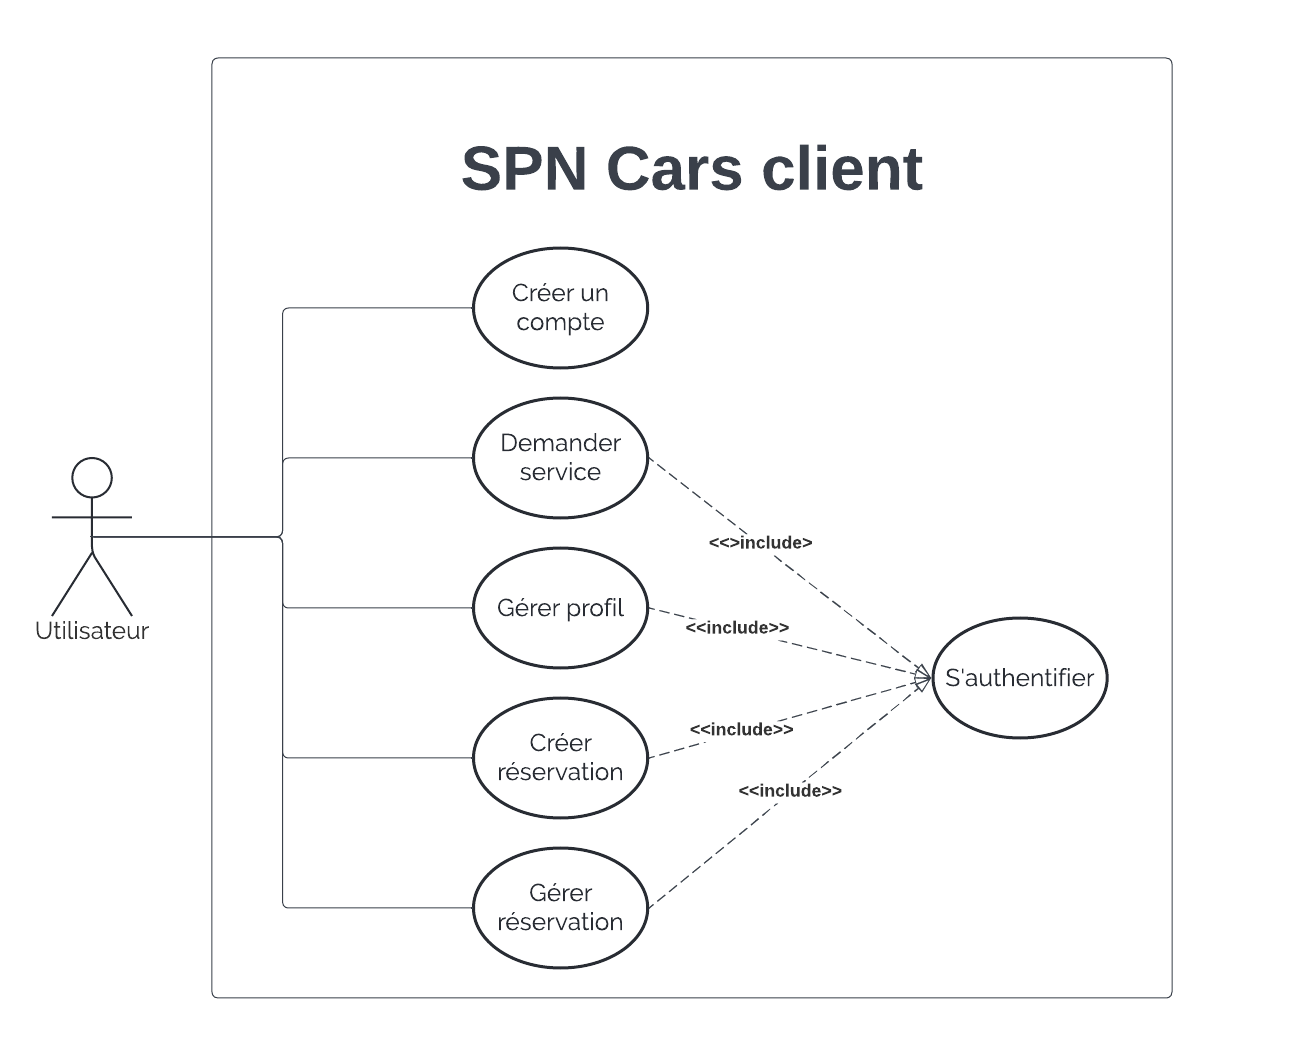
\includegraphics[height=0.5\textheight]{uml/use_cases.png}
    \vspace{1cm}
    \captionsetup{justification=centering}

    \caption{Diagramme de cas d'utilisation}
    \label{fig:use_case_diag}
\end{figure}
\subsection{Diagramme de classes}
\begin{figure}[H]
    \centering
    \rotatebox[origin=c]{-90}{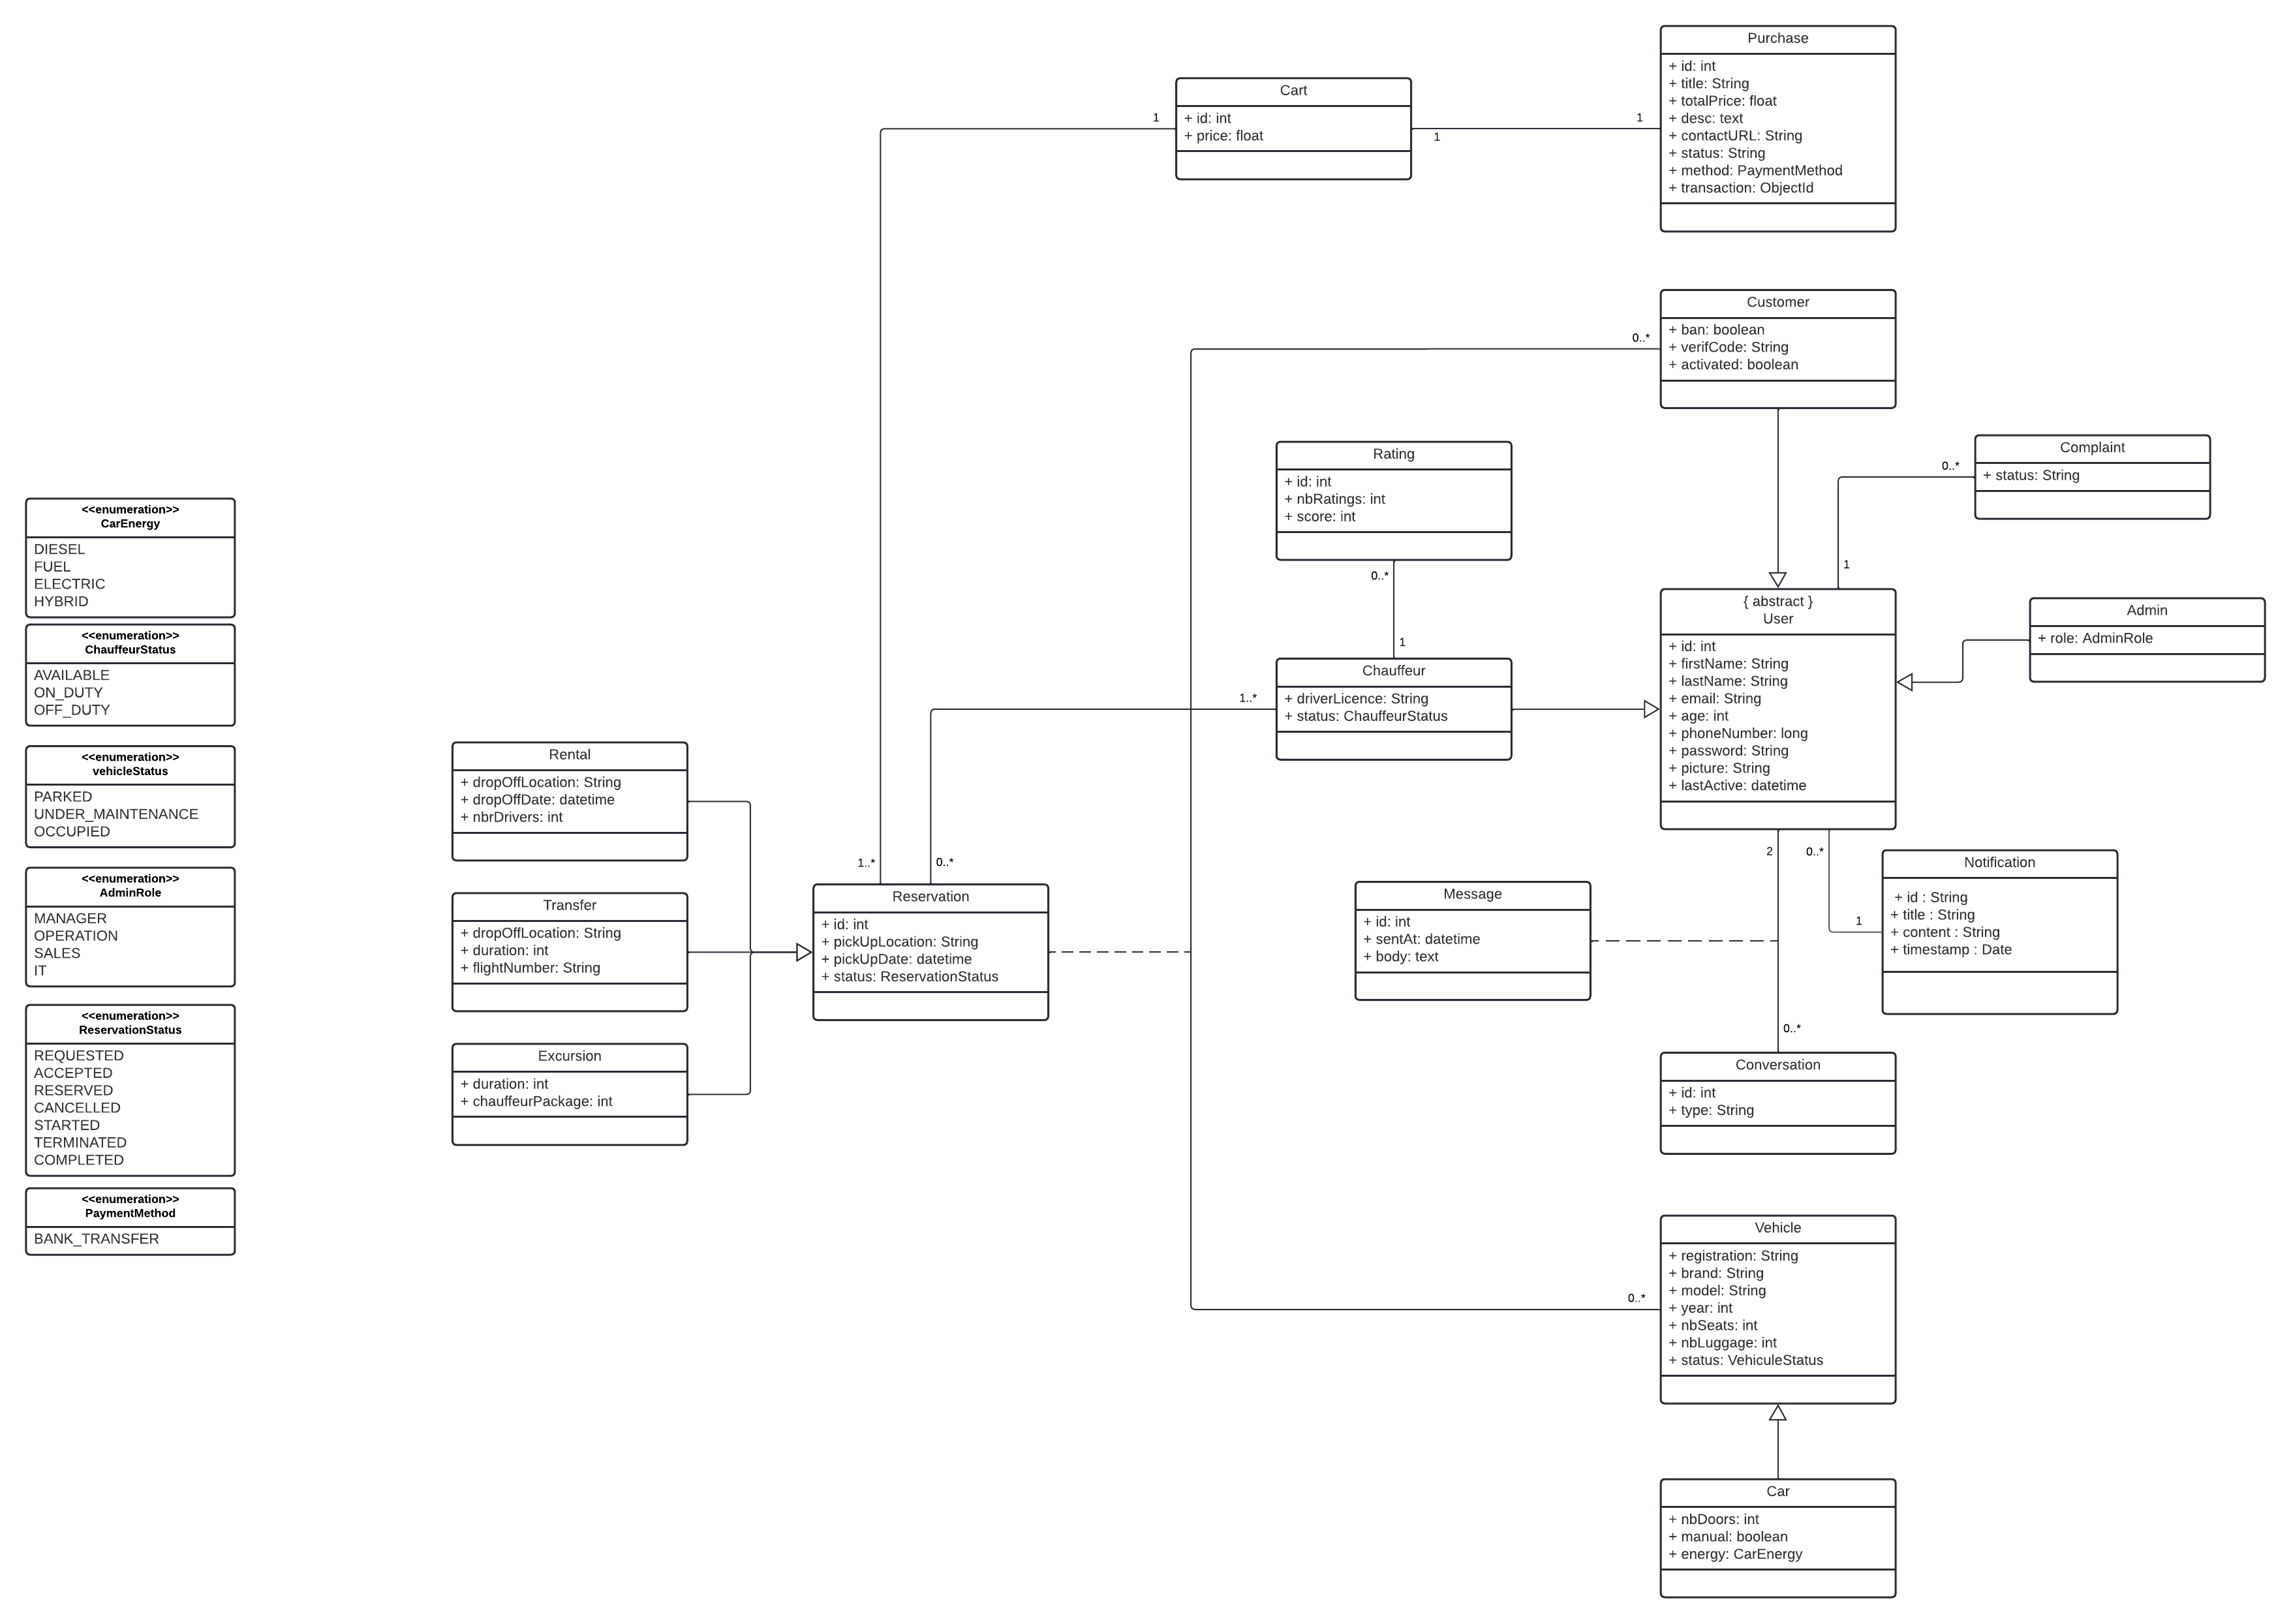
\includegraphics[width=0.9\textheight,height=\textwidth]{uml/class_diag.png}}
    \vspace{1cm}
    \captionsetup{justification=centering}

    \caption{Diagramme de classe}
    \label{fig:class_diag}
\end{figure}
\clearpage
\subsection{Diagrammes de séquences}
Les diagrammes de séquences sont le moyen qui permettent de décrire d'une manière détaillée les différents cas d'utilisation
\subsubsection{Création de compte}
\begin{figure}[H]
    \centering
    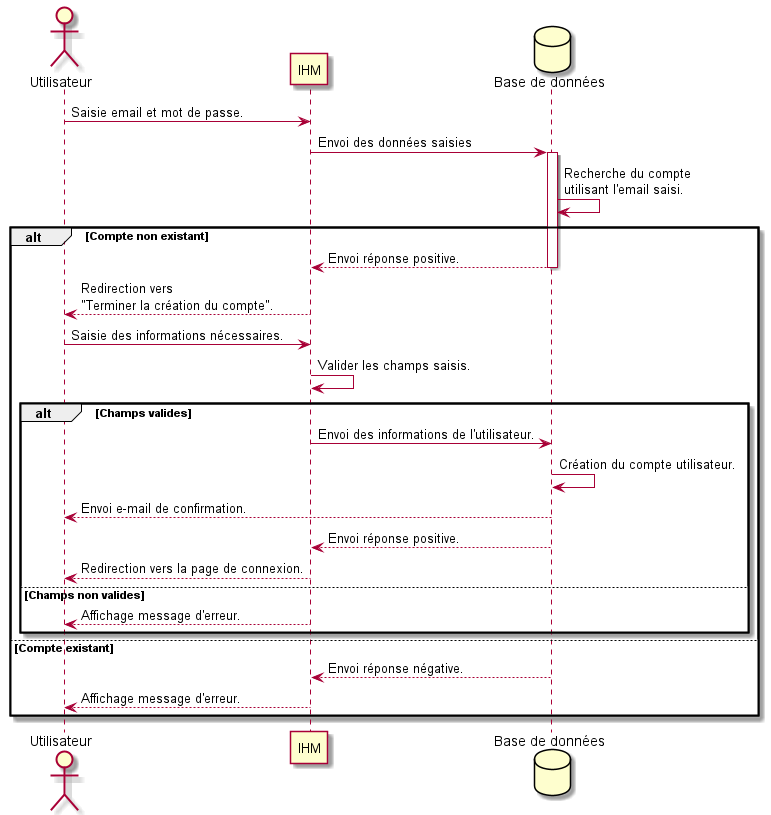
\includegraphics[width = \textwidth]{uml/register_email.png}
    \vspace{1cm}
    \captionsetup{justification=centering}

    \caption{Diagramme de séquence : Création de compte avec E-mail et mot de passe.}
    \label{fig:seq_register_email}
\end{figure}
\begin{figure}[H]
    \centering
    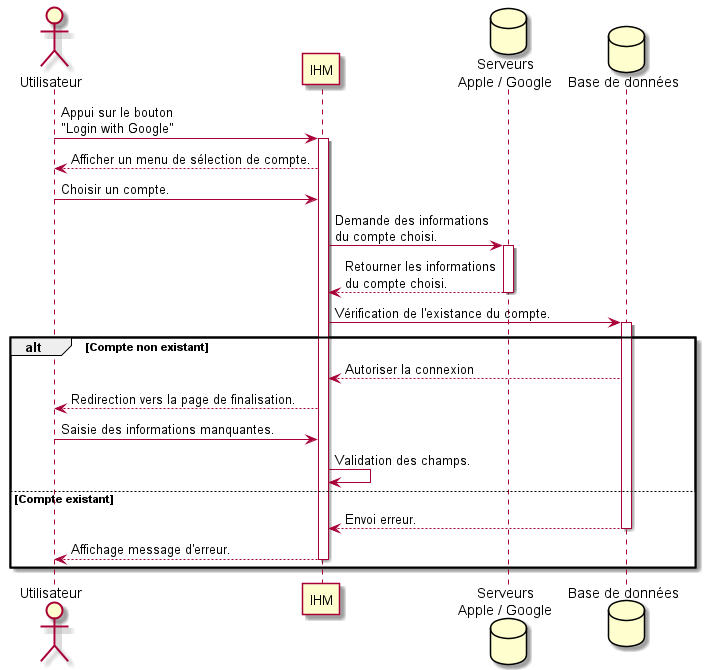
\includegraphics[width = \textwidth]{uml/apple_google.png}
    \vspace{1cm}
    \captionsetup{justification=centering}

    \caption{Diagramme de séquence : Création de compte avec Un compte Google / Apple.}
    \label{fig:seq_register_apple_google}
\end{figure}
\subsubsection{Authentification}
\begin{center}
    \begin{figure}[H]
        \centering
        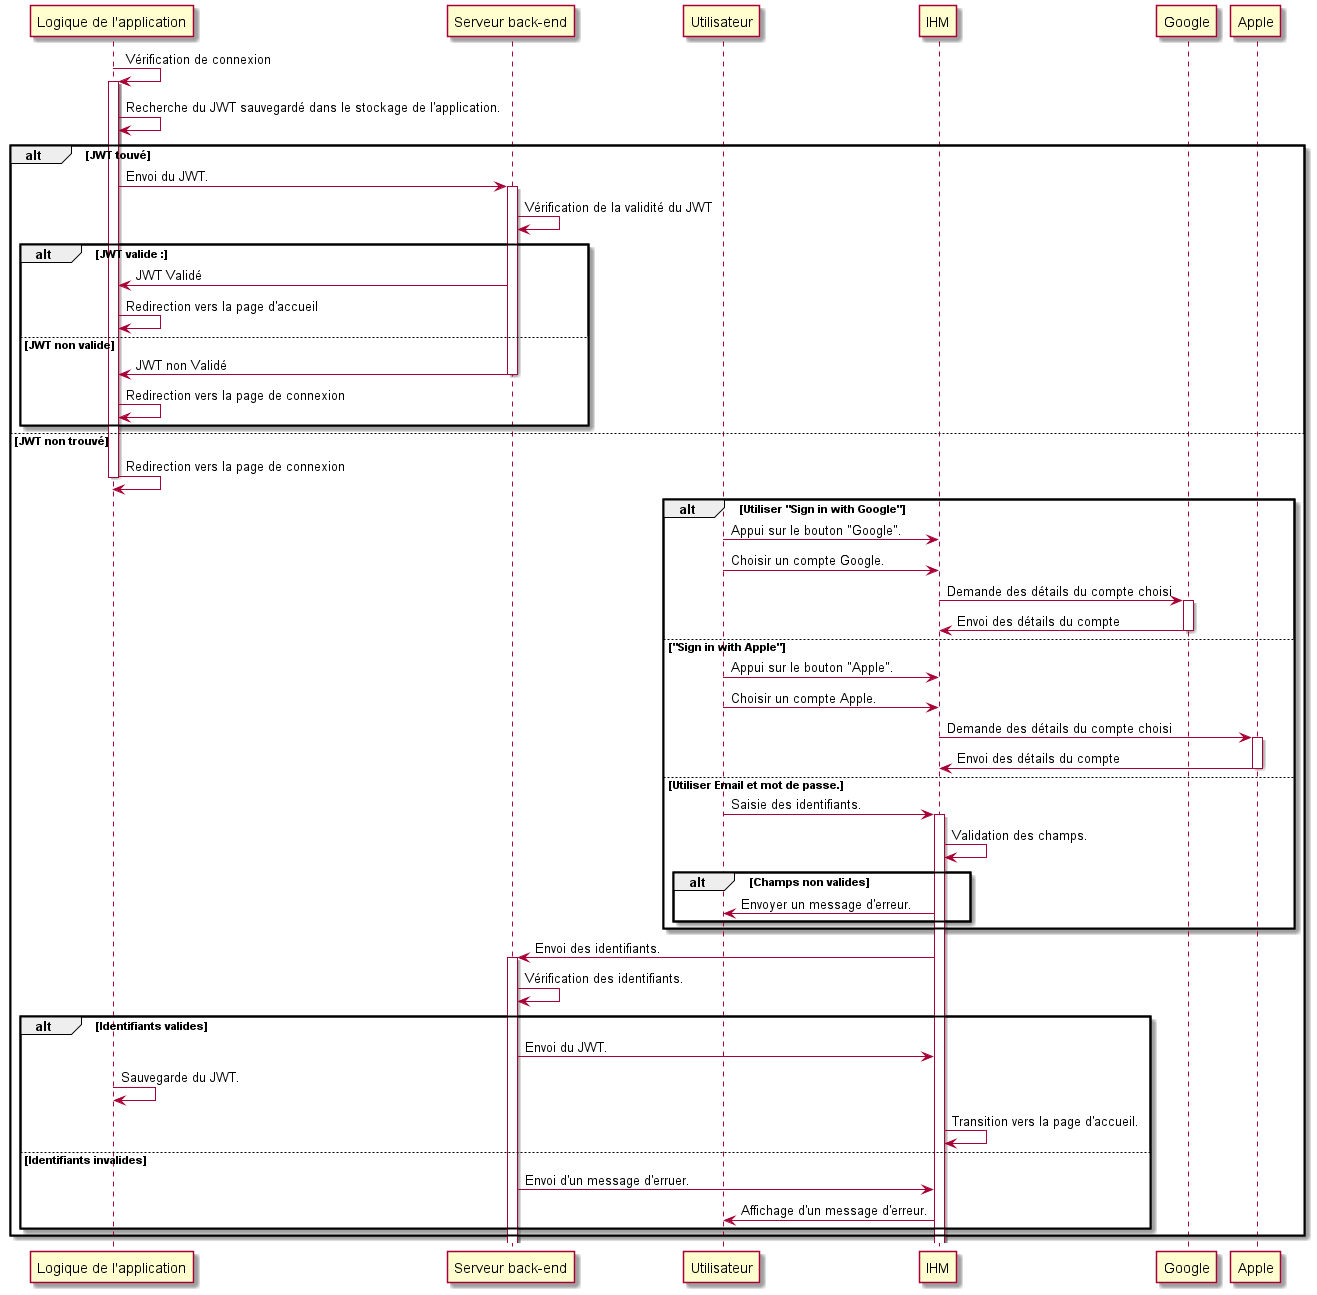
\includegraphics[width = \textwidth]{uml/Authentification.png}
        \vspace{1cm}
        \captionsetup{justification=centering}

        \caption{Diagramme de séquences: Authentification.}
        \label{fig:seq_auth}
    \end{figure}
\end{center}
\subsubsection{Page d'accueil}
\begin{figure}[H]
    \centering
    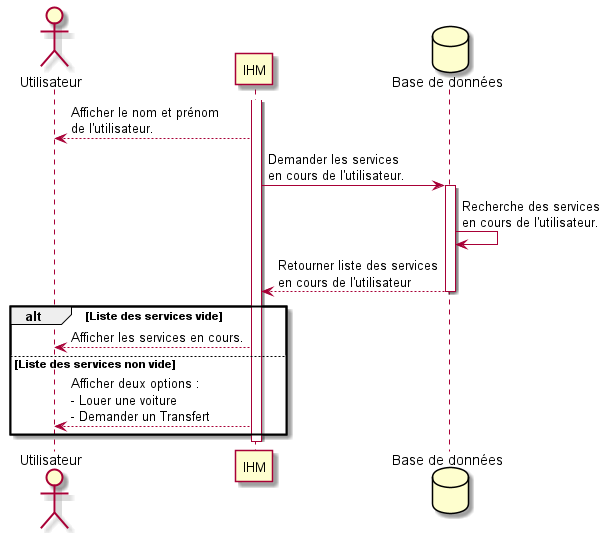
\includegraphics[width=\textwidth]{uml/home.png}
    \vspace{1cm}
    \caption{Diagramme de séquences : Page d'accueil.}
    \label{fig:seq_home}
\end{figure}
% \subsubsection{Gestion de profil}
\subsubsection{Demander un service}
\begin{figure}[H]
    \centering
    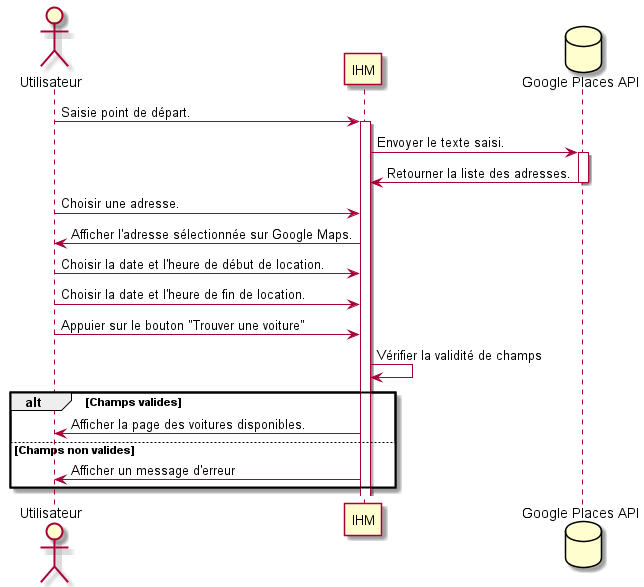
\includegraphics[width = \textwidth]{uml/rent a car.png}
    \vspace{1cm}
    \captionsetup{justification=centering}

    \caption{Diagramme de séquences: Demander une location.}
    \label{fig:seq_location}
\end{figure}
\vspace{1cm}
\begin{figure}[H]
    \centering
    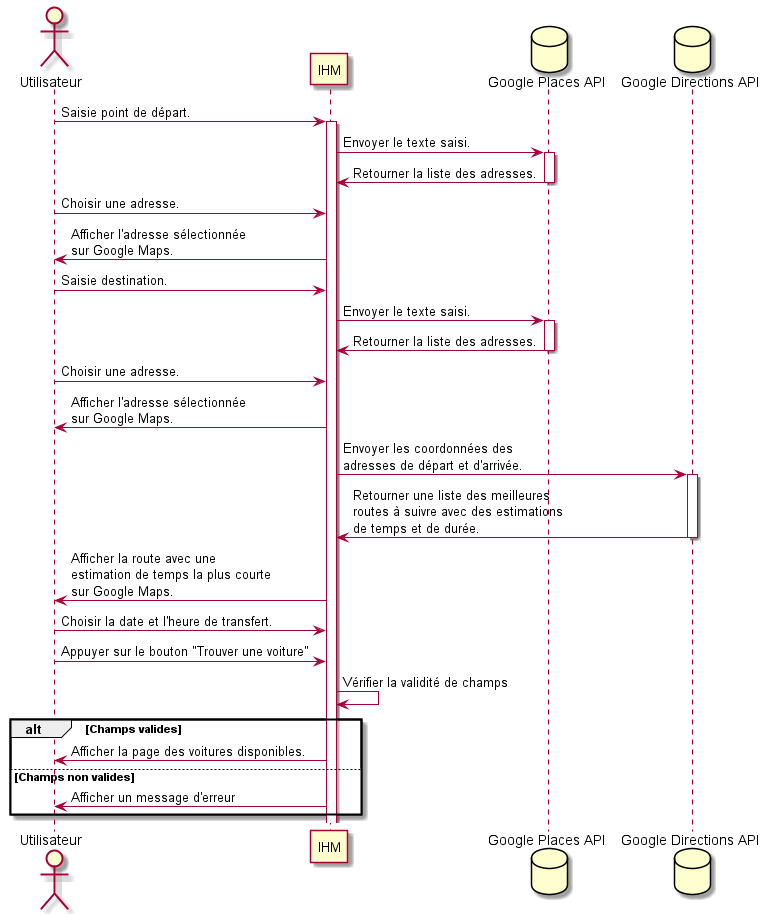
\includegraphics[width = \textwidth]{uml/transfert.png}
    \vspace{1cm}
    \captionsetup{justification=centering}

    \caption{Diagramme de séquences: Demander un transfert.}
    \label{fig:seq_transfert}
\end{figure}
\subsubsection{Affichage des voitures disponibles}
\begin{figure}[H]
    \centering
    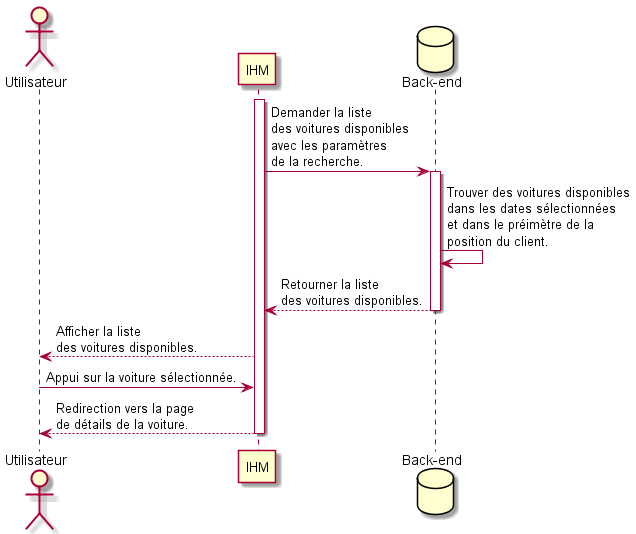
\includegraphics[width = \textwidth]{uml/choisir voiture.png}
    \vspace{1cm}
    \captionsetup{justification=centering}

    \caption{Diagramme de séquences : Choisir une voiture}
    \label{fig:seq_car_select}
\end{figure}
\subsubsection{Signature numérique de contrat de location}
\begin{figure}[H]
    \centering
    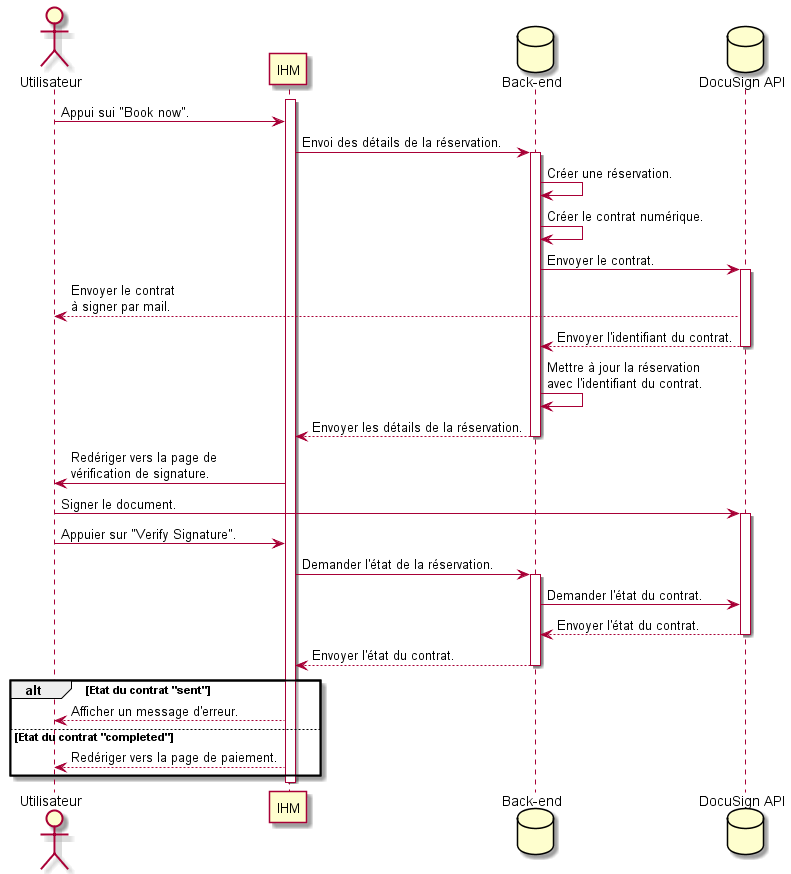
\includegraphics[width = \textwidth]{uml/docusign.png}
    \captionsetup{justification=centering}
    \caption{Diagramme de séquences : Envoi du contrat de location.}
    \label{fig:seq_location_contract}
\end{figure}
\subsubsection{Paiement en ligne}
\begin{figure}[H]
    \centering
    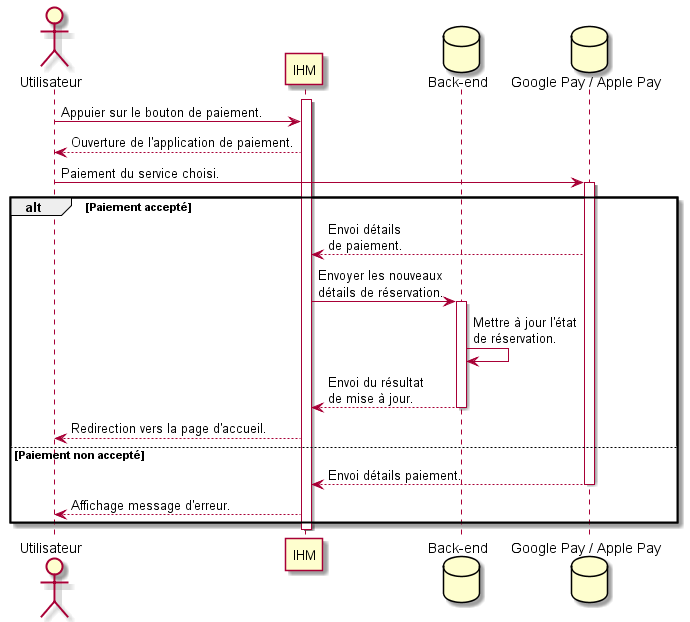
\includegraphics[width = \textwidth]{uml/payment.png}
    \captionsetup{justification=centering}
    \caption{Diagramme de séquences: Paiement des services.}
    \label{fig:seq_payment}
\end{figure}
\subsubsection{Localiser une voiture}
\section{UI/UX Design}
Avant de passer au développement de l'application, il faut créer d'abord les prototypes des interfaces utilisateur. \\
\noindent Cette étape est nécessaire pour tester plusieurs approches dans les interfaces de l'application, s'assurer d'offrir une expérience optimale pour l'utilisateur. \\
\noindent Suite à une collaboration avec l'équipe de design UI/UX, les interfaces suivantes ont été créées.
\vspace{1cm}
\begin{multicols}{2}
    \begin{figure}[H]
        \centering
        
\includegraphics[width=0.25\textwidth]{ui_screenshots/Guide.png}
        \vspace{1cm}
        \captionsetup{justification=centering}

        \caption{Première page.}
        \label{fig:start_page}
    \end{figure}
    \begin{figure}[H]
        \centering
        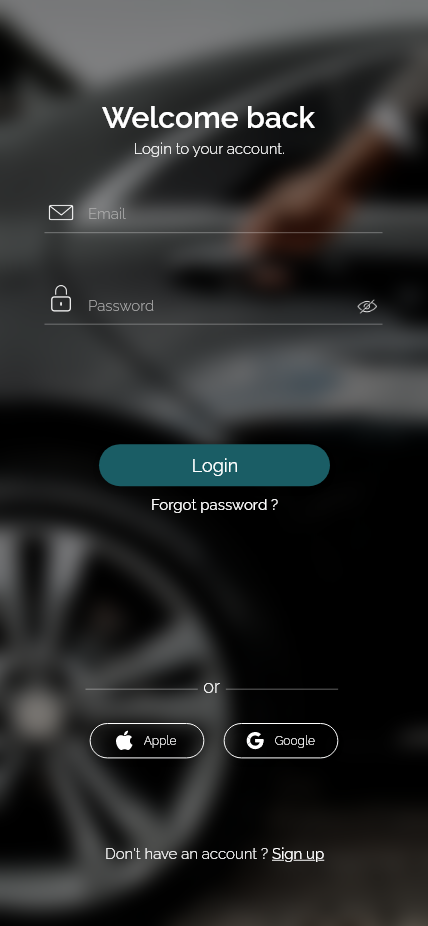
\includegraphics[width=0.25\textwidth]{ui_screenshots/sign in.png}
        \vspace{1cm}
        \captionsetup{justification=centering}

        \caption{Page de connexion.}
        \label{fig:sign_in_page}
    \end{figure}
\end{multicols}
% \newpage
\begin{multicols}{2}
    \begin{figure}[H]
        \centering
        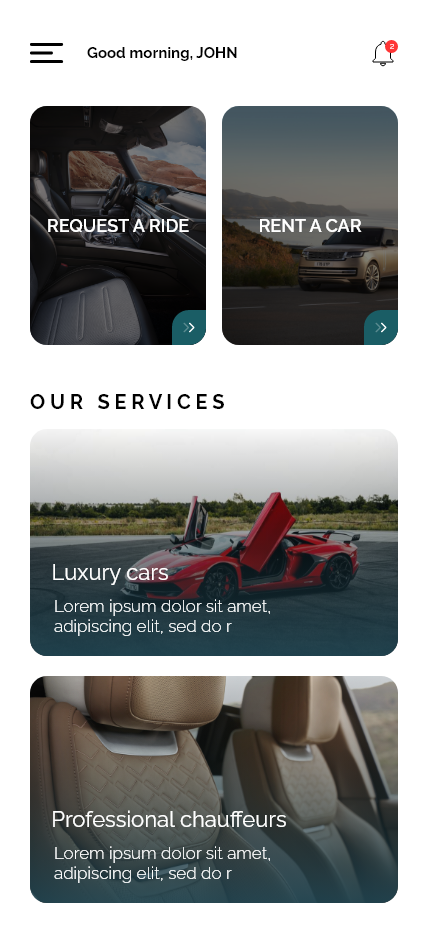
\includegraphics[width=0.25\textwidth]{ui_screenshots/No Active trip.png}
        \vspace{1cm}
        \captionsetup{justification=centering}

        \caption{\centering Page d'accueil.}
        \label{fig:no_active_trip}
    \end{figure}
    \begin{figure}[H]
        \centering
        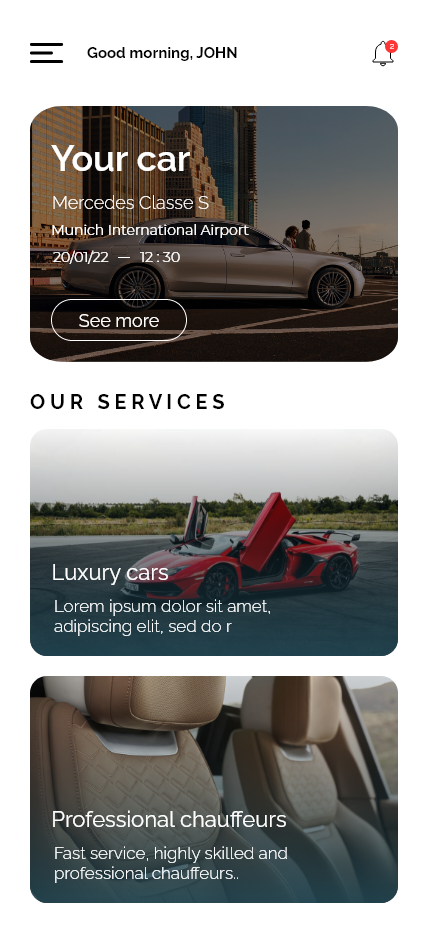
\includegraphics[width=0.25\textwidth]{ui_screenshots/Active trip.png}
        \vspace{1cm}
        \captionsetup{justification=centering}

        \caption{\centering Page d'accueil lors d'un transfert en cours.}
        \label{fig:active_trip}
    \end{figure}
\end{multicols}
\clearpage
\begin{multicols}{2}
    \begin{figure}[H]
        \centering
        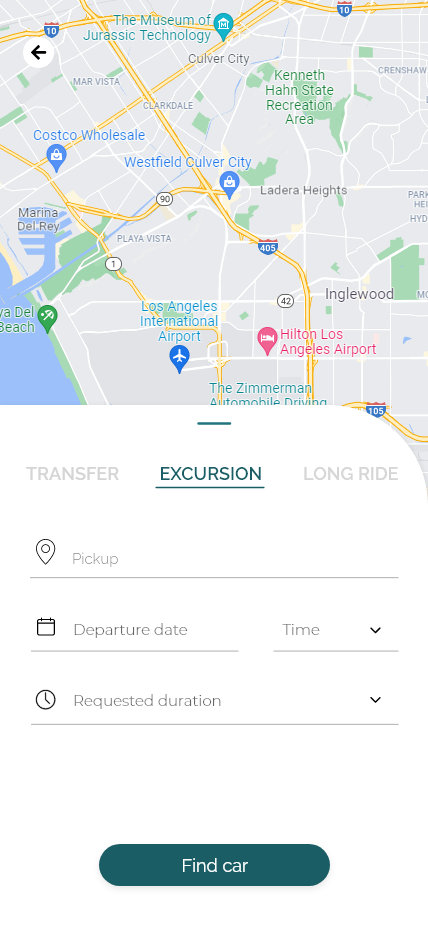
\includegraphics[width=0.25\textwidth]{ui_screenshots/Excursion.png}
        \vspace{1cm}
        \captionsetup{justification=centering}

        \caption{\centering Sélection de type de transfert.}
        \label{fig:trip_select}
    \end{figure}
    \begin{figure}[H]
        \centering
        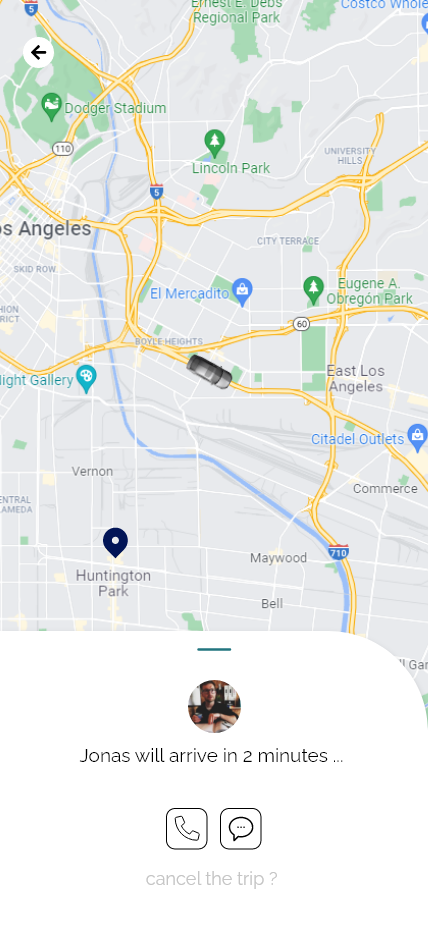
\includegraphics[width=0.25\textwidth]{ui_screenshots/Map view.png}
        \vspace{1cm}
        \captionsetup{justification=centering}

        \caption{\centering Suivi de la position actuelle du chauffeur avec la voiture.}
        \label{fig:follow_driver}
    \end{figure}
\end{multicols}
\begin{multicols}{2}
    \begin{figure}[H]
        \centering
        \includegraphics[width=0.25\textwidth]{ui_screenshots/Available cars – 1.png}
        \vspace{1cm}
        \captionsetup{justification=centering}

        \caption{\centering Liste de voitures disponibles.}
        \label{fig:available_cars}
    \end{figure}
    \begin{figure}[H]
        \centering
        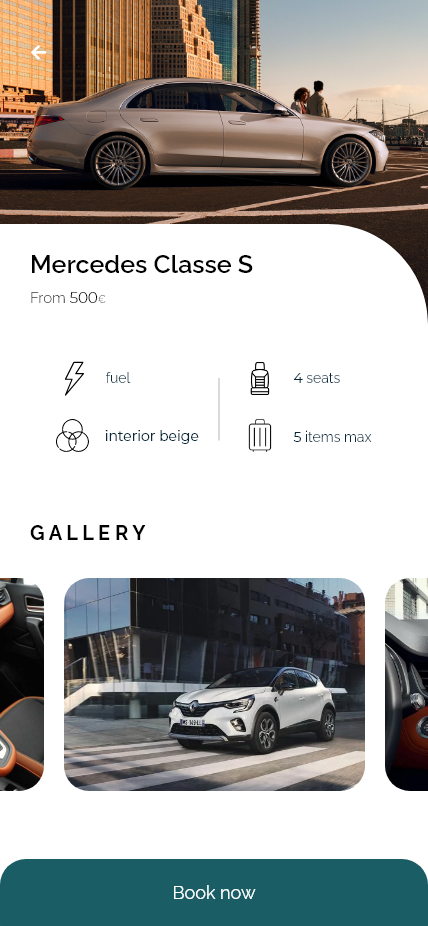
\includegraphics[width=0.25\textwidth]{ui_screenshots/Car details.png}
        \vspace{1cm}
        \captionsetup{justification=centering}

        \caption{\centering Détails de la voiture sélectionnée.}
        \label{fig:car_details}
    \end{figure}
\end{multicols}
\vspace{1cm}
\begin{figure}[H]
    \centering
    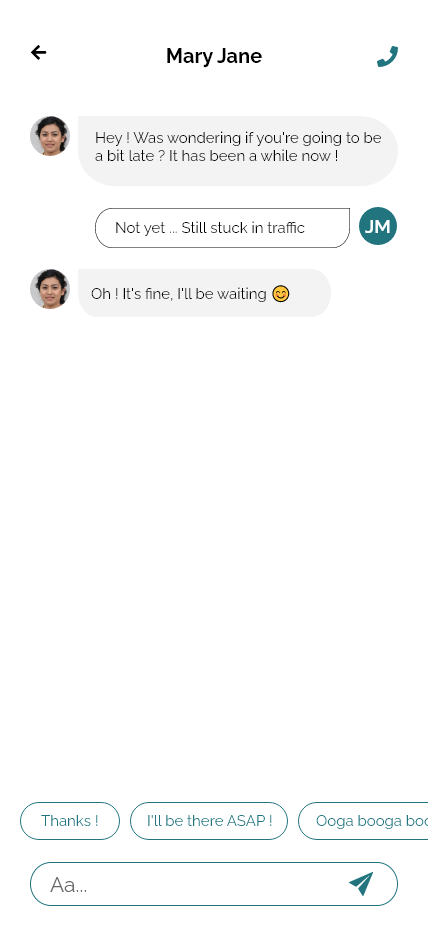
\includegraphics[width=0.25\textwidth]{ui_screenshots/DMs.png}
    \vspace{1cm}
    \caption{\centering Messagerie instantannée avec le chauffeur.}
    \label{fig:dms}
\end{figure}
\section{Technologies et outils utilisés}
Comme cette application sera une application mobile, il est nécessaire que la performance soit la priorité lors du développement. C'est pourquoi on a choisi les technologies suivantes pour offrir une application rapide, performante, facile à utiliser.\\
\noindent Ses différentes technologies sont classifiés dans trois domaines principalement : Conception des interfaces graphiques, développement de l'application, et développement du back-end de l'application.\\
\subsection{Flutter}
\vspace{1cm}
\begin{figure}[H]
    \centering
    
\includegraphics[width=0.25\textwidth]{flutter.png}
    \vspace{1cm}
    \captionsetup{justification=centering}

    \caption{Logo Flutter}
    \label{fig:flutter_logo}
\end{figure}
\textit{\textbf{Flutter}} \cite{flutter} est un kit de développement (SDK) open-source créé par Google et publié en 2017.\\
\noindent Flutter permet de créer des application mobiles (Android / iOS), web et meême desktop (Windows / Linux / MacOS), avec une seule base de code en Dart, un langage de programmation développé aussi par Google. \\
\noindent Flutter présente plusieurs avantages qui permettent de créer des applications mobiles performantes et réduit aussi le coût et le temps de développement nécessaires, grâce au langage de programmation utilisé \textit{\textbf{Dart}} qui est très facile à maîtriser et qui offre plusieurs avantages, dont le plus important la fonctionnalité de <<\textit{\textbf{Hot Reload}}>> qui permet de recharger l'application et afficher les changements sur l'écran sans passer par la recompilation du code source.
\subsection{Express JS}
\vspace{1cm}
\begin{figure}[H]
    \centering
    
\includegraphics[width=0.25\textwidth]{express.png}
    \vspace{1cm}
    \captionsetup{justification=centering}

    \caption{Logo Express}
    \label{fig:express_logo}
\end{figure}
\textit{\textbf{Express JS}} \cite{expressjs} est un framework back-end gratuit et open-source pour NodeJS. Créé par TJ Holowaychuk, la première version publique d'Express JS a été introduite au public en 2010.\\
Express JS est un framework minimaliste, très léger pour garantir une performance optimale et une exécution rapide. Ce framework est aussi très flexible, même s'il fournit que quelques fonctionnalités, grâce à \textit{\textbf{NPM}}, le gestionnaire de packets de NodeJS, il peut être complété par plusieurs librairies disponibles.\\
\noindent Grâce à son minimalisme et facilité d'implémentation, ExpressJS est utilisé par plusieurs par nombreuses sociétés dans le monde, pour développer tout type d'applications, parmi ses sociétés il y a des géants de technologies tels que \textit{\textbf{IBM}}, \textit{\textbf{Uber}}, et plusieurs autres.
\subsection{MongoDB}
\vspace{1cm}
\begin{figure}[H]
    \centering
    
\includegraphics[width=0.25\textwidth]{mongo.png}
    \vspace{1cm}
    \captionsetup{justification=centering}

    \caption{Logo MongoDB}
    \label{fig:mongo_logo}
\end{figure}
\textit{\textbf{MongoDB}} \cite{mongodb} , est un système de gestion de base de données NoSQL, orientée documents. Une base de données NoSQL est utilisée pour le stockage de volumes massifs de données, elle se distingue des des bases de données relationnelles par sa flexibilité et ses performances.\\
\noindent Le système MongoDB est développé par la société qui porte le même nom en 2007. Cette entreprise travaillait sur un système de cloud computing à données largement réparties.\\
\noindent Il est depuis devenu l'un des systèmes de gestion de base de données les plus utilisées, notamment pour des sites web très populaires tels que : \textit{\textbf{SourseForge.net}}, \textit{\textbf{eBay}} et \textit{\textbf{The New York Times}}.\\
\noindent Contrairement à une base de données relationnelle SQL traditionnelle, MongoDB ne repose pas sur des tableaux et des colonnes. Les données sont stockées sous forme de collections et de documents.
Les documents sont des paires de valeurs / clés servant d'unité de données de base. Les collections quant à elles contiennent des ensembles de documents et de fonctions. Elles sont l'équivalent des tableaux dans les bases de données relationnelles classiques.
\subsection{Firebase}
\vspace{1cm}
\begin{figure}[H]
    \centering
    
\includegraphics[width=0.25\textwidth]{firebase.png}
    \vspace{1cm}
    \captionsetup{justification=centering}

    \caption{Logo Firebase}
    \label{fig:firebase_logo}
\end{figure}
\textit{\textbf{Firebase}} \cite{firebase} est une plateforme créée en 2011, puis acquise et développée par Google en 2014. Firebase facilite la création de back-end à la fois scalable et performant.\\
\noindent L'objectif de firebase est d'offrir aux professionnels et aux particuliers un moyen d'éviter l'engagement dans un processus complexe de création et de maintenance d'une architecture serveur.\\
\noindent Firebase offre des API intuitives regroupées dans un SDK unique. Ces API permettent de gagner du temps et de réduire le nombre d'intégrations qu'on doit gérer dans l'application.\\
\noindent Firebase offre plusieurs services que tout le monde peut utiliser gratuitement grâce à sa politique <<pay as you go>> qui nécessite le paiement de ses services seulement si l'utilisation des ressources dépasse le quota du plan gratuit offert. Les services de Firebase les plus utilisés sont :
\begin{itemize}
    \item \textbf{Firestore}:\\ Une base de données NoSQL, bénéficiant d'un hébergement cloud et permettant le stockage et la synchronisation de données des untilisateurs.
    \item \textbf{Fireabse Authentification}:\\ Un SDK prêt et facile à exploiter qui permet de d'authentifier les utilisateurs en offrant plusieurs méthodes d'authentification tels que Google, Apple, Facebook, Email et mot de passe, numéro de téléphone et plusieurs d'autres méthodes pour assurer l'authentification de l'utilisateur.
    \item \textbf{Firebase Cloud Messaging}:\\ Permet de connecter plusieurs périphériques au serveur dans les meilleures conditions (fiabilité et économie de batterie). Ce service permet de recevoir et envoyer des notification sur les différentes plateformes (Web / iOS / Android). Avec Firebase Cloud Messaging, il est possible aussi d'assurer un service de messagerie instantanée entre les utilisateurs.
\end{itemize}
\subsection{Adobe Xd}
\vspace{1cm}
\begin{figure}[H]
    \centering
    
\includegraphics[width=0.25\textwidth]{xd_logo.png}
    \vspace{1cm}
    \captionsetup{justification=centering}

    \caption{Logo Adobe Xd}
    \label{fig:xd_logo}
\end{figure}
\textit{\textbf{Adobe Xd}} \cite{adobe_xd} est un outil de conception et modélisation des interfaces utilisateur des applications web et mobiles, développé par Adobe Inc.\\
\noindent Grâce aux outils fournis par Adobe Xd, la conception, l'amélioration et la rectification des interfaces graphiques et l'expérience de l'utilisateur de l'application sera plus facile, plus rapide et plus efficace.
\noindent Dans le cadre de ce projet, Adobe Xd a été utilisé pour la création des prototypes des interfaces graphiques, qui seront, par la suite, construits en application mobile à l'aide de Flutter.
\subsection{Git}
\vspace{1cm}
\begin{figure}[H]
    \centering
    
\includegraphics[width=0.25\textwidth]{git.png}
    \vspace{1cm}
    \captionsetup{justification=centering}

    \caption{Logo Git}
    \label{fig:git_logo}
\end{figure}
\textit{\textbf{Git}} \cite{git} est un système de contrôle de version open-source créé en 2005 par \textit{\textbf{Linus Torvalds}}, le créateur du noyau du système d'exploitation Linux.\\
\noindent Git permet de gérer les ajouts et changements apportés au code source de manière tracée. Ainsi, si une erreur est commise, les développeurs peuvent revenir en arrière et comparer les versions antérieures du code, ce qui leur permet de corriger l'erreur tout en minimisant les perturbations pour tous les membres de l'équipe.
\subsection{Swagger}
\vspace{1cm}
\begin{figure}[H]
    \centering
    
\includegraphics[width=0.25\textwidth]{swagger.png}
    \vspace{1cm}
    \captionsetup{justification=centering}

    \caption{Logo Swagger}
    \label{fig:swagger_logo}
\end{figure}
\textit{\textbf{Swagger}} \cite{swagger} est un langage permettant de créer une description des API Restful à l'aide de JSON. A l'aide de ses outils Open-Source, Swagger permet de concevoir, créer et décrire des API REST.\\
\noindent Swagger est créer en 2011 par Tony Tam, cofondateur du site de dictionnaires Wordnik, suite à un besoin d'automatisation de documentation de l'API qui est devenue de plus en plus frustrante. Juste après sa création, le projet Swagger est devenu open-source en septembre 2011.\\
\noindent Swagger est maintenant maintenu par la société \textit{\textbf{SmartBear Software}} qui, en novembre 2015, de créer une organisation appelée \textit{\textbf{OpenAPI initiative}} dont diverses entreprises tels que Google, IBM et Microsoft sont les membres fondateurs.\\
\section*{Conclusion}
A travers ce chapitre, on a établi la conception de l'application SPN-Cars: On a dégager les besoins fonctionnels et non fonctionnels, qui, à travers eux on a pu créer les diagrammes de cas d'utilisation, les diagrammes de classes, et les diagrammes de séquences. Suite au développement de ces diagrammes, on a passé vers l'étape de conception des interfaces utilisateur. Toutes ces différentes étapes ont permit de choisir les technologies et outils qui seront utilisés pour la création de cette application.\\
Une fois les différents aspects de l'applications sont bien définis, on passera vers la phase de réalisation où on appliquera les diagrammes et interfaces développés dans ce chapitre pour produire cette application.